\lab{Algorithms}{Fourier Transform Extensions}{Fourier Transform Extensions}
\objective{Learn about two particular extensions of the Fourier Transform: cepstral analysis and the two-dimensional
FFT.}

The ideas at the basis of the one dimensional Fourier Transform that you explored in previous labs can be
extended in many ways to a variety of different settings. One way to extend the Fourier Transform, which is
a linear theory, is to compose it with non-linear operations. This is the basis of Cepstral Analysis, which we
will briefly discuss and then apply to the study of sound signals. Another way to generalize the basic
Fourier Transform is to move into higher dimensions, which we do when exploring the two-dimensional FFT.
Although we only address these two topics in this lab, keep in mind that the Fourier Transform and its
generalizations are central to the mathematical field of harmonic analysis as well as myriad applications
in physics, engineering, statistics, and other fields.

\subsection*{The Fourier Transform in Python}
SciPy includes the module \li{scipy.fftpack} that contains several useful and easy to use functions
for calculating the Fourier Transform and its variants. Refer to the documentation to learn about
the available tools. This module does not, however, take full advantage of the optimizations provided
by the FFTW library written in the C programming language. We recommend PyFFTW, a Python module that
is built around FFTW. For convenience, the submodule \li{pyfftw.interfaces.scipy_fftpack} mimics the
\li{scipy.fftpack} module, containing the same functions with the same interfaces, just higher-performance.

\subsection*{Cepstral Analysis and Mel-Frequency Cepstral Coefficients}
\begin{figure}
\centering
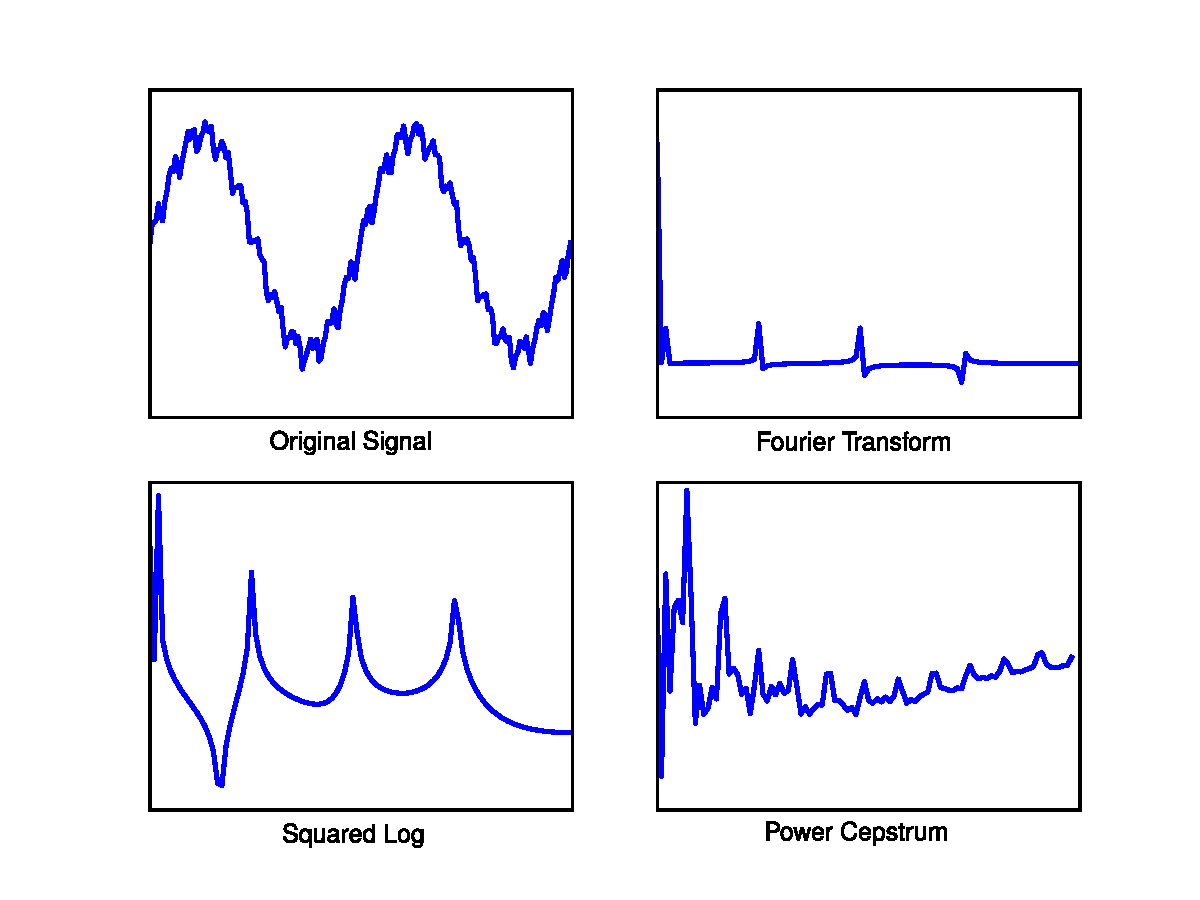
\includegraphics[width=\textwidth]{PowerCepstrum.pdf}
\caption{Example of the steps in calculating the Power Cepstrum.}
\label{fourierext:pc}
\end{figure}
When analyzing complex sound signals such as speech or music, the simple spectral information provided by
the Fourier Transform by itself is often insufficient. For example, while the Fourier Transform does reveal
the prominent frequencies in a sound signal, it does a poor job of highlighting the more subjective
tonal qualities, or \emph{timbre}, of the signal (qualities that help us distinguish between different singers
or different musical instruments).

Cepstral analysis was developed to partially redress this situation, and it provides a collection of signal
processing techniques that go beyond the basic Fourier Transform. The basic idea is to analyze the
\emph{cepstrum} of a signal as opposed to the \emph{spectrum} (which is the approach of basic Fourier
analysis). There are various ways to define the cepstrum, and they all involve composing the Fourier
Transform with non-linear operations. Given a signal $f(t)$, the \emph{Power Cepstrum} is defined by
$$
\left|\mathcal{F}^{-1}\{\log(|\mathcal{F}(f(t))|^2)\}\right|^2,
$$
where $\mathcal{F}$ denotes the Fourier transform. The \emph{Complex Cepstrum} is defined by
$$
\mathcal{F}\{\log(\mathcal{F}(f(t)))+j2\pi m\},
$$
where $j$ is the imaginary unit and $m$ is a carefully chosen integer, and the \emph{Real Cepstrum}
is defined by
$$
\mathcal{F}^{-1}\{\log(|\mathcal{F}(f(t))|^2)\}.
$$
The usefulness of each type of Cepstrum is determined by the theoretical setting or the application.
The complex Cepstrum has the interesting and useful property of transforming the convolution operation
into an additive operation. In particular, if $f$ and $g$ are signals with corresponding complex
cepstra $f'$ and $g'$, and if $*$ represents the convolution operation, we have
$$
f * g \rightarrow f' + g'.
$$
The reason for this relies on the fact that convolution can be converted to multiplication by
the Fourier transform, and when the logarithm is applied it becomes addition.
This is useful when trying to separate two signals that have been convolved with each other, such as
a source and a filter, a problem known as \emph{deconvolution}.
Other uses for the various cepstra include fundamental pitch detection in speech signals, voice
identification, and analysis of signals containing echoes.

As a side note, the field of Cepstral analysis comes with its own distinctive jargon, including ``cepstrum",
``quefrency", ``liftering", and ``alanysis". These are derived, respectively, from ``spectrum",
``frequency", ``filtering", and ``analysis". See Figure \ref{fourierext:pc} for an example of the Power
Cepstrum.

\begin{problem}
Write a function \li{powerCepstrum} that accepts a one-dimensional array $f$ and computes the
power cepstrum of $f$, according to the definition given above.
\end{problem}

We now turn our attention to the computation of \emph{Mel-frequency cepstral coefficients} (MFCCs), which
are data useful in signal classification problems such as
speech recognition and automatic musical instrument classification.

Expressed in simple terms, calculating the MFCCs involves splitting the signal up into a sequence of
short segments called \emph{frames}, calculating a variant of the Power Cepstrum for each one,
and reducing the dimensionality of the results through a process called \emph{binning}. What we are
left with is a collection of numbers that summarizes each of the frames, with the hope that these
numbers capture important spectral and timbral information about the original signal.

Suppose we have a sound signal 2 seconds long sampled at a standard rate of 44100 Hz, which means the
signal has 88200 entries. The  MFCCs are obtained through a series of steps, which are outlined
as follows:
\begin{figure}
\centering
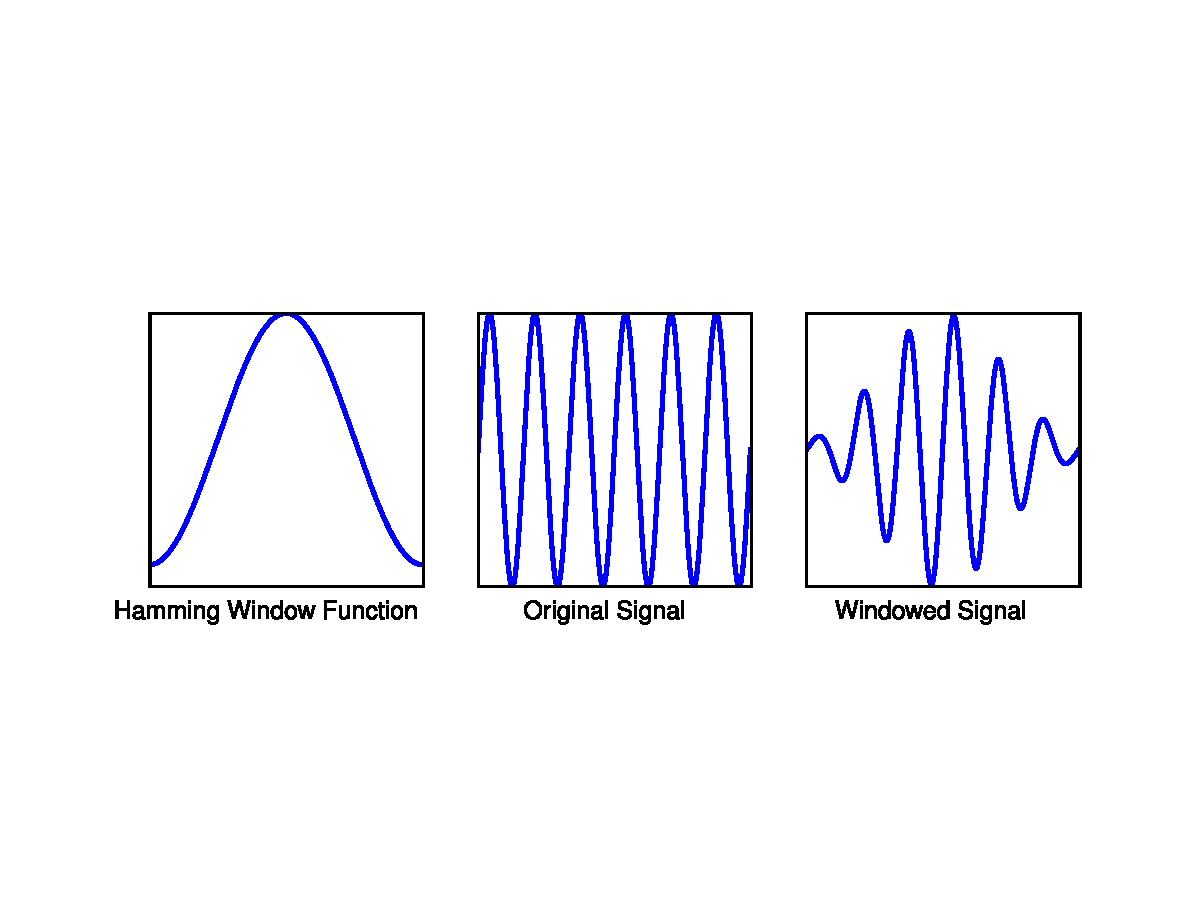
\includegraphics[width=\textwidth]{Hamming.pdf}
\caption{The Hamming Window.}
\label{fourierext:ham}
\end{figure}
\begin{itemize}
\item \emph{Windowing}. This refers to splitting up the original signal into a sequence of overlapping
short segments called frames, and then applying a so-called \emph{window-function}, which scales down
the edges of the frames.

In the particular case at hand, we wish to split up the signal into frames approximately 30 ms in
duration, with adjacent frames overlapping by 20 ms. This means splitting our signal into $198$ frames,
each frame containing $1323$ values from the original signal, overlapping $882$ values with each frame
immediately preceding and following it. We then multiply each frame by a \emph{Hamming} window of length
1323 (we have provided the code to calculate a Hamming window of a given length). See Figure
\ref{fourierext:ham} for an example of the Hamming window applied to a signal.

\begin{problem}
Write a function \li{window} that accepts a 2-second sound signal with sample rate 44100, and
returns a list of the 198 windowed frames calculated as in the description above.
\end{problem}

\item \emph{Pre-emphasis and Power Spectrum}. For each frame $\tilde{f}$, we next apply
a filtering process known as \emph{pre-emphasis} used to improve the signal-to-noise ratio as follows:
\begin{equation*}
\widehat{f}_{n} = \tilde{f}_{n} - 0.95 \tilde{f}_{n-1}
\end{equation*}
for $n = 1,\ldots,1322$, and $\widehat{f}_0 = \tilde{f}_0$ (in Python, this can be done in one line of code using vectorization).
We then compute the \emph{power spectrum} of the result, which is the square of the magnitude of the
Fourier transform.

\begin{problem}
Write a function \li{powerSpectrum} that accepts a frame (one dimensional array of length 1323) and
applies pre-emphasis and then computes the power spectrum of the result. In this computation,
pad the frame with zeros so that it is of length 2048 when computing the fourier transform. This
can be done by using the keyword argument \li{n = 2048} when calling
\li{pyfftw.interfaces.scipy_fftpack.fft}. Furthermore, only return the first 1025 entries of the result,
since the remaining entries are just a mirror image of the first half.
\end{problem}

\item \emph{Mel Scale}. The Mel Frequency scale is based on human perception of pitch. It maps frequency
in Herz to a slightly distorted scale where equal distances between values correspond to equal perceived
differences in pitch. Using matrix multiplication, we will map the power spectrum of each frame to
mel scale bins, thereby reducing the dimensionality of the frames and representing them in a scale
more closely aligned with human perception of pitch. See Figure \ref{fourierext:mel} for a depiction
of the Mel Scale as well as a typical Mel filterbank, which defines the binning process.

We have provided the code to calculate the required mel scale
matrix (use 40 filters, with FFT length 2048 and sample rate 44100).
Before we perform this multiplication, however, we first want to prevent underflow problems. We
therefore want to set all values of the power spectrum below a certain threshold to that threshold value.
For our purposes, we will set this threshold value to \li{1e-100}.

\begin{figure}
\centering
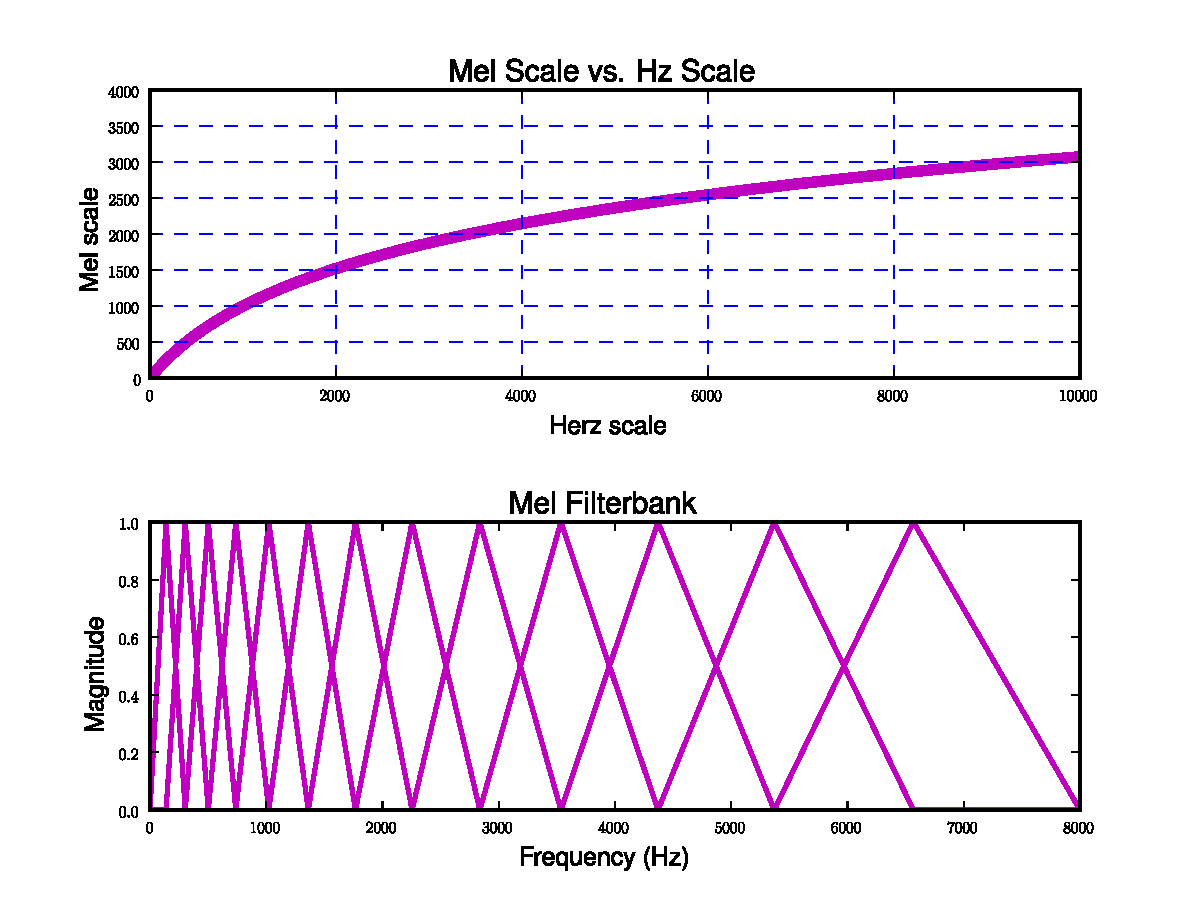
\includegraphics[width=\textwidth]{melScale.pdf}
\caption{The Mel Scale and Mel Filterbank.}
\label{fourierext:mel}
\end{figure}

\item \emph{Discrete Cosine Transform}. To complete the process, we take the Discrete Cosine Transform
of the \emph{logarithm} of the resulting mel scale power spectrum frames, multiply the result by 0.25, and retain only entries 2
through 11 (yielding an array of length 10), since these are the entries that contain most of desired
information. The Discrete Cosine Transform is very similar to the Fourier Transform, but only uses
cosine functions rather than a combination of cosine and sine functions in the series expansion of the
signal. In many cases, sums of cosine functions alone can more efficiently represent signal than
sums of both sine and cosine functions, so the Discrete Cosine Transform is preferred in these cases.
\end{itemize}
After this process, we should end up with a list of 198 arrays, each of length 10. These are our MFCCs,
which can then be used in various classification algorithms.

\begin{problem}
Write a function \li{extract} which accepts an array of length 88200 (representing a two second sound sample
with rate 44100 Hz), and returns an array of shape (198,10), where each row gives the calculated MFCCs for
a particular windowed frame of the original signal. Use your previous solutions as you see fit, and try to
avoid unnecessary looping.
\end{problem}

\subsection*{The 2-dimensional FFT}
\begin{figure}
\centering
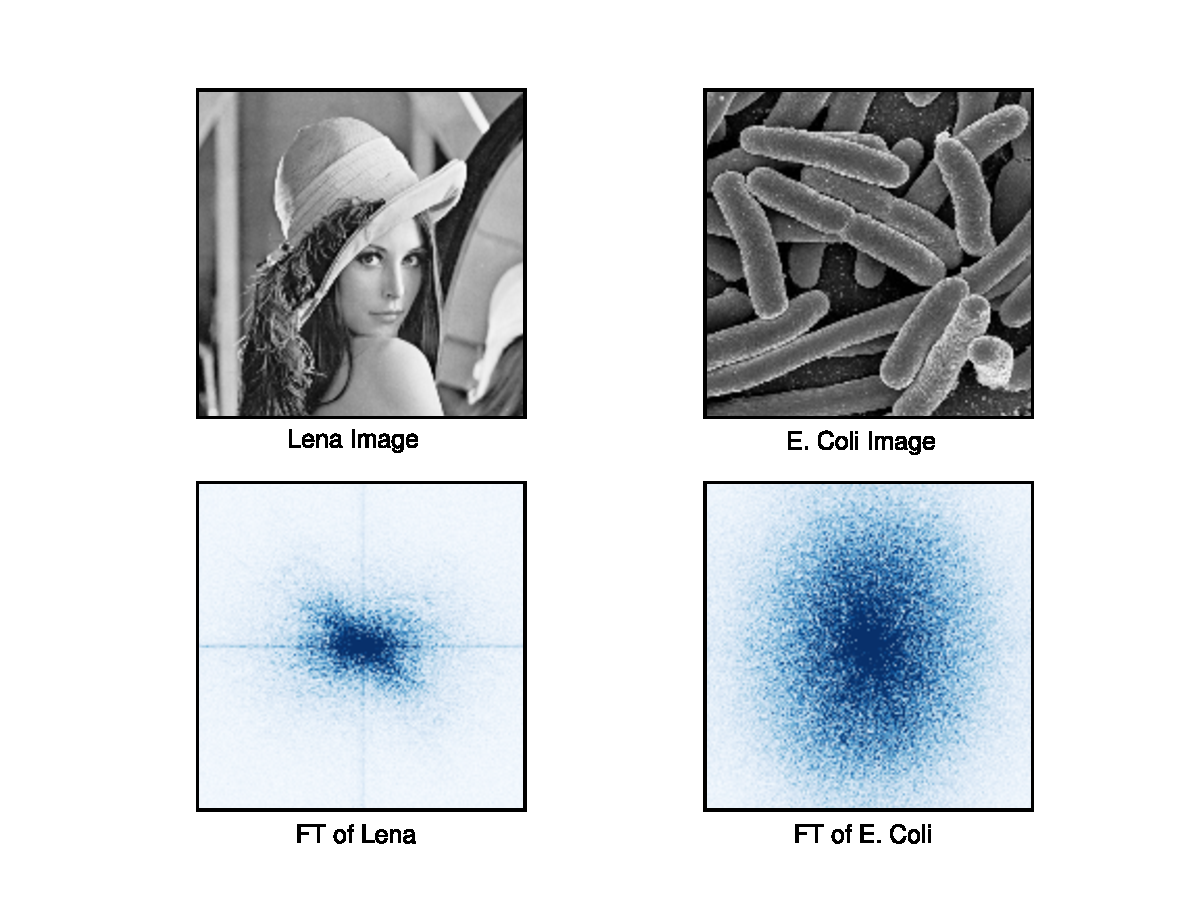
\includegraphics[width=\textwidth]{2dfft.pdf}
\caption{The 2D Fourier Transform Applied to Images.}
\label{fourierext:2dfft}
\end{figure}
You know how to calculate the Fourier Transform for one-dimensional signals. In fact, the theory of
Fourier Transforms may be readily extended to any number of dimensions.
Computationally, the problem reduces to performing the one-dimensional Fourier Transform iteratively
along each of the dimensions. We will focus on calculating the Fourier Transform of two-dimensional
matrices. In this setting, we think of the matrices not as functions of time, but rather as functions of
space. One we have the 2-dimensional Fourier Transform, we can perform many useful operations for
denoising, compression, edge-detection, image enhancement, and more.

Given a matrix $A$, we first calculate the one-dimensional Fourier Transform of each column, storing the
result column-wise in an array the same shape as $A$. We then calculate the Fourier Transform of each
row of this resulting array, and this yields the two-dimensional Fourier Transform of $A$.

Calculating the two-dimensional inverse Fourier Transform is done in a similar fashion, but in the
oppositive order: first calculate the inverse Fourier Transform of the rows, then the columns.

\begin{problem}
Write a function \li{fft2} that accepts a two-dimensional array as input and returns the two-dimensional
Fourier Transform of the input. You may use built-in methods to calculate the one-dimensional Fourier
Transform.

Write another function \li{ifft2} that accepts a two-dimensional array as input and returns the two-
dimensional inverse Fourier Transform. Once again,  you may use built-in methods to calculate the
one-dimensional inverse Fourier Transform.
\end{problem}

We can visualize the two-dimensional Fourier Transform as follows:
\begin{lstlisting}
import numpy as np
import pyfftw
from matplotlib import pyplot as plt

# In the following, F is the output of 2dFFT
# Shift values in F for optimal visualization
F_s = pyfftw.interfaces.scipy_fftpack.fftshift(F)

# Convert all values to nonnegative real numbers
F_mag = np.abs(F_s)

# Scale the values, then amplify
amp = 1000 # you may want to test other values for amp
F_mag *= amp/F_mag.max()

# Set values larger than 1 to 1
F_mag[F_mag > 1] = 1

# Plot the result
plt.imshow(F_mag, plt.cm.Greys)
plt.show()
plt.clf()
\end{lstlisting}
See Figure \ref{fourierext:2dfft} for an example. The visualization indicates
the relative strengths of various frequencies in the original image.
As you will notice, the largest values of the fourier transform are concentrated
near the center of each visualization, which tells us that the original images are
composed mostly of smaller frequencies. The presence of higher frequencies is indicated
by values farther away from the center of the visualization, and these account for the
finer details of the original images.
%Does anyone know of a better way to intuitively describe these visualizations?

